\documentclass[11pt]{beamer}
\usepackage[utf8]{inputenc}
\usepackage[spanish]{babel}
\usepackage{amsmath}
\usepackage{amsfonts}
\usepackage{amssymb}
\usepackage{graphicx}
\usepackage{lipsum}
\usepackage{ragged2e}
\usepackage{hyperref}
\usepackage{float}
\usepackage{url}
\usepackage{hyperref}
\usetheme{Madrid}
\newcommand{\celda}[1]{
	\begin{minipage}{2.5cm}
		\vspace{5mm}
		#1
		\vspace{5mm}
	\end{minipage}
}

\author[Arocutipa \& Coaquira]{FACULTAD DE INGENIERÍA, PRODUCCIÓN Y SERVICIOS\\Fundamentos de la Programación}
\title[UNSA]{MODULARIZACIÓN}
\date{AGOSTO DEL 2020} 
\subtitle{UNIVERSIDAD NACIONAL DE SAN AGUSTÍN}
\logo{
\includegraphics[scale=0.05]{../../../../Pictures/sm.png}}
\institute[EPIS]{
	\inst{Alumnos:}
		Arocutipa Gutierres Luis Edgar\\Coaquira Mamani Cesar Paul\\
		\vspace{2mm}
	\inst{Profesor:}
		Escobedo Quispe Richart Smith 
}

\AtBeginSection[]
{
	\begin{frame}<beamer>{Contenido}
		\tableofcontents[currentsection,currentsubsection]
	\end{frame}
}


\begin{document}
	
	\begin{frame}
		\maketitle
	\end{frame}

	\begin{frame}{Contenido}
		\tableofcontents
	\end{frame}

	\section{Introducción}
		\begin{frame}{Introducción
}
			\justifying
			Los algoritmos están presentes en todas nuestras acciones, para resolver situaciones cotidianas tales como cruzar una calle, preparar una taza de té o leer un libro.
			\begin{figure}[hbtp]
		\centering
		
\includegraphics[scale=0.8]{../../../../Pictures/im1.png}
		\end{figure}
		\end{frame}
	
	\section{Conceptos iniciales}
		\begin{frame}{Conceptos iniciales}
			\justifying
\vfill
\textbf{Módulos o subprogramas:} Son cada una de las acciones que ejecutamos en nuestro algoritmo y que luego vamos a desarrollar.\\
\vfill
 \textbf{Funciones:} Una función es un subprograma invocado desde el programa principal (o desde otra función) que ejecuta una tarea determinada y retorna el control al programa o función que la invocó.\\
\end{frame}
	
	\section{Función o método definido según el programador}
		
\begin{frame}{Función o método definido según el programador}
			\justifying
\textbf{Estructura General de una función:}
\begin{figure}[hbtp]
		\centering
		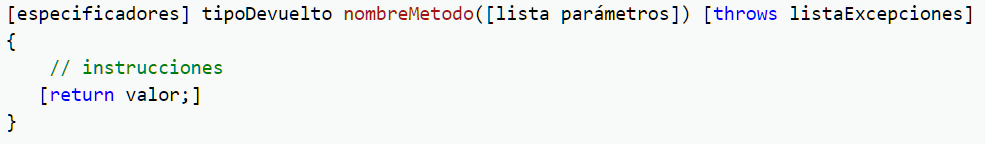
\includegraphics[scale=0.5]{../../../../Pictures/im6.png}
		\end{figure}
	\textbf{1. Especificadores}
	\vfill\textbf{2. TipoDevuelto}\\
	\vfill\textbf{3. NombreMétodo}\\
	\vfill\textbf{4. Lista de Parámetros}(opcional)\\
	\vfill\textbf{5. throws listaExcepciones}\\
	\vfill\textbf{6. return}\\
\end{frame}
\begin{frame}{Función o método definido según el programador}
			\justifying
\textbf{Pasos para implementar un método} 
\vfill
1.     Describir lo que el método debe hacer.\\
\vfill
2.     Determinar las entradas del método, es decir, lo que el método recibe.\\
\vfill
3.     Determinar los tipos de datos de las entradas.\\
\vfill
4.     Determinar lo que debe devolver el método y el tipo del valor devuelto.\\
\vfill
5.     Escribir las instrucciones que forman el cuerpo del método.\\
\vfill
6.     Prueba del método: diseñar distintos casos de prueba.\\
\vfill
\textbf{Invocar a una función:} Cuando se llama a un método, la ejecución del programa pasa al método y cuando éste acaba, la ejecución continúa a partir del punto donde se produjo la llamada.\\
\begin{figure}[hbtp]
		\centering
		\textbf{Ejemplo}
		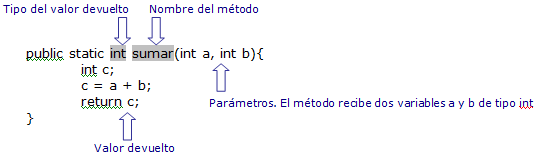
\includegraphics[scale=0.4]{../../../../Pictures/im2.png}
		\end{figure}
\end{frame}

		\begin{frame}{Funciones definidas según el programador}
			\justifying
\textbf{Funciones de tipo void:} Este tipo se utiliza para                                          indicar que una función no retorna ningún valor.
\begin{figure}[hbtp]
		\centering
		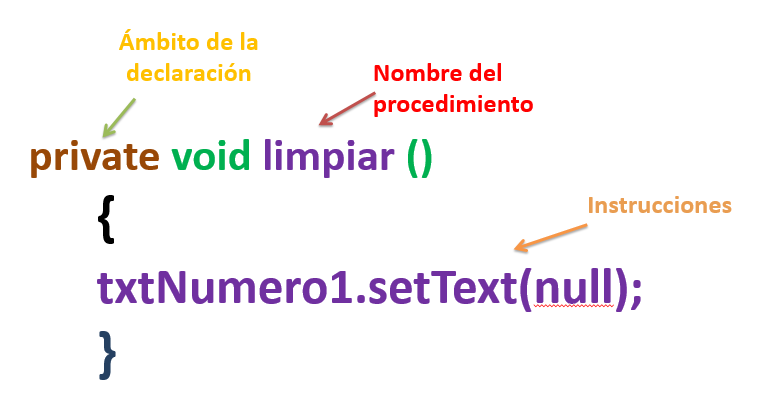
\includegraphics[scale=0.15]{../../../../Pictures/im7.png}
		\end{figure}

		\textbf{Métodos no estáticos: } Este tipo de métodos suelen ser usados más frecuentemente que los métodos estáticos.
La diferencia radica en que estos métodos solo son corridos en un objeto y no en toda la clase como pasaba anteriormente.
		\begin{figure}[hbtp]
		\centering
		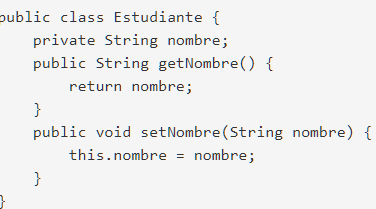
\includegraphics[scale=0.5]{../../../../Pictures/im9.png}
		\end{figure}
\end{frame}
\begin{frame}{Funciones definidas según el programador
}
			\justifying
		\textbf{Método estático:}Pertenecen a la clase(no están asociados a un objeto particular de la clase, por lo tanto no pueden acceder a las variables de instancia de un objeto(las cuales pertenecen a objetos particulares.
		\vfill \textbf{Constructor(this):} Son métodos especiales que sirven para inicializar el estado de un objeto cuando lo creamos con el operador new.\\ \vfill -Su nombre ha de coincidir con el nombre de la clase. \\
		\vfill -Por definición no devuelve nada.\\
		\vfill -La palabra reservada this permite acceder al objeto sobre el que se ejecuta el método.\\
\begin{figure}[H]
				\centering
				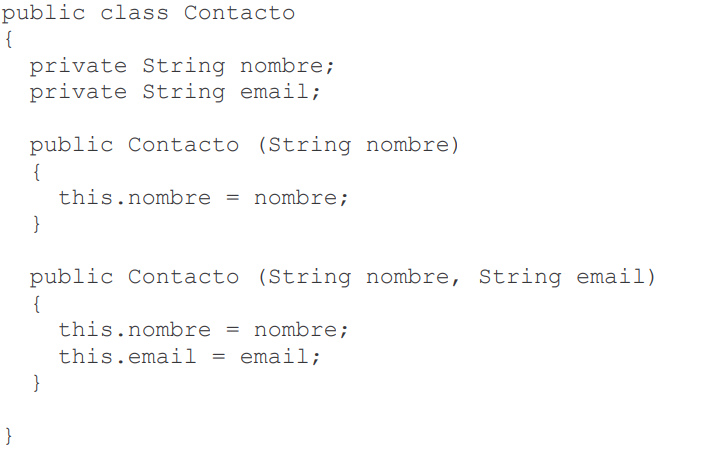
\includegraphics[scale=0.3]{../../../../Pictures/im30.png}
			\end{figure}
		\end{frame}
		
	
	
	\section{Alcance de las variables
}
		\begin{frame}{Alcance de las variables
}
			\justifying
		\textbf{Variable de Instancia:}Es una variable definida para las instancias de una clase (cada objeto tiene su propia copia de la variable de instancia y abarca los métodos no estáticos de una clase.
		\vfill \textbf{    -Cuando es privada:} Todos los métodos pueden acceder al valor almacenado.\\
		\vfill \textbf{    -Cuando es pública:} Se puede acceder a ella desde cualquier lugar que disponga de una referencia a un objeto.\\

			\vfill
	       \textbf{Variable Local:} Comienza en su declaración y termina donde termina el bloque de código({}) que contiene la declaración

\begin{figure}[H]
				\centering
				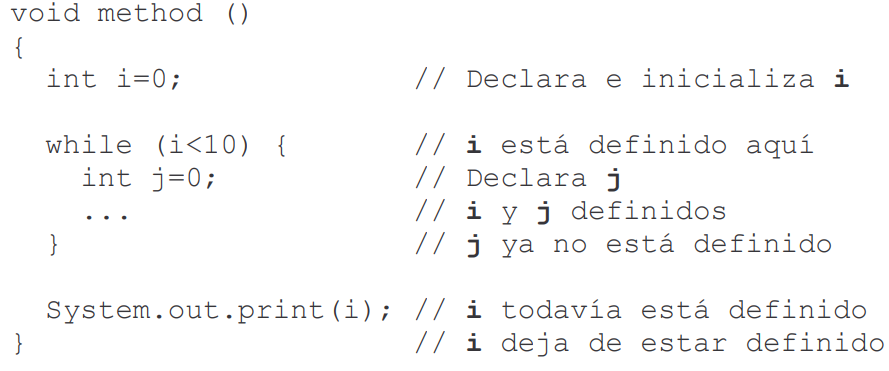
\includegraphics[scale=0.3]{../../../../Pictures/im11.png}
			\end{figure}
		\end{frame}
		
		
		\section{Ejercicios}
	\begin{frame}{Ejercicios
}
			\justifying
			\textbf{Ejercicio 01-Básico: }Programa que da la Suma y Resta de dos Números. 
			\begin{figure}[hbtp]
		\centering
		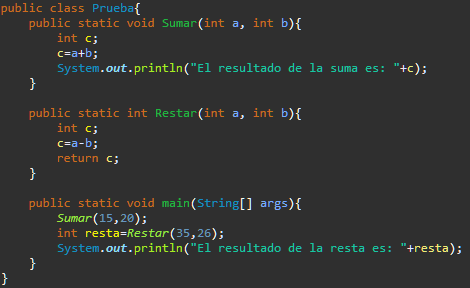
\includegraphics[scale=0.8]{../../../../Pictures/im22.png}
		\end{figure}
		\end{frame}
		\begin{frame}{Ejercicios
}
			\justifying
			\textbf{Ejercicio 02-Básico: }Programa que muestra la tabla de ´´un número ingresado por teclado
			\begin{figure}[hbtp]
		\centering
		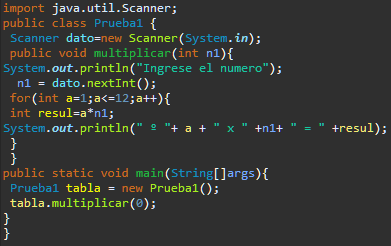
\includegraphics[scale=0.8]{../../../../Pictures/im23.png}
		\end{figure}
		\end{frame}
		
		\begin{frame}{Ejercicios
}
			\justifying
			\textbf{Ejercicio 03-Avanzado: }Programa que imprime la cantidad de euros que tiene en una cuenta según ingresa o retira dinero. Clase Principal:
			\begin{figure}[hbtp]
		\centering
		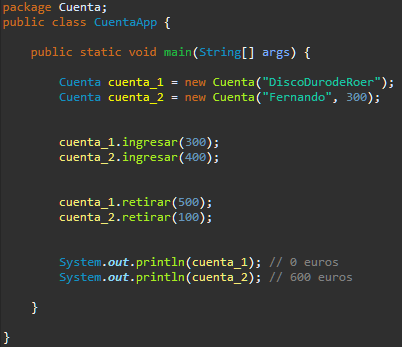
\includegraphics[scale=0.7]{../../../../Pictures/im24.png}
		\end{figure}
		 
		\end{frame}
		\begin{frame}{Ejercicios
}
			\justifying
			\textbf{Ejercicio 03-Avanzado: }Clase Cuenta:
			\begin{figure}[hbtp]
		\centering
		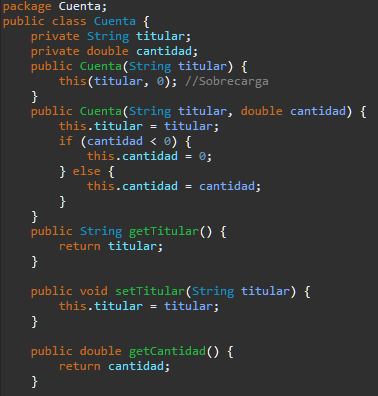
\includegraphics[scale=0.55]{../../../../Pictures/im25.png}
		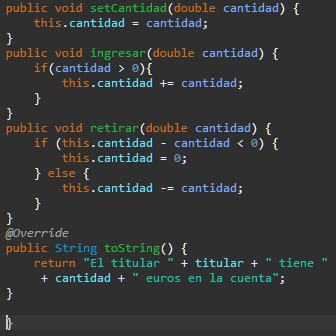
\includegraphics[scale=0.55]{../../../../Pictures/im26.png}
		
		\end{figure}
		 
		\end{frame}
		
		
		
		
\section{Referencias}

\begin{frame}{Referencias}

\begin{thebibliography}{10}
	
	\beamertemplatearticlebibitems
	% imagen de libro
	
	\bibitem{Author}
	Ing. Pablo Augusto Sznajdleder
	\newblock{\em Algoritmos a fondo : con implementaciones en C y Java . - 1a ed. - }.
	\newblock{\textbf{Fuente: }\url{https://www.academia.edu/40129651/Algoritmos_a_fondo_Con_implementaciones_en_C_y_Java}}
	
	\beamertemplateonlinebibitems
	\bibitem{Author}
	Programación Java/Métodos en Java
	\newblock{\em Enrique García Hernández}.
\newblock{\textbf{Fuente: }\url{https://puntocomnoesunlenguaje.blogspot.com/2012/04/metodos.html?fbclid=IwAR3yp0IKgRNqyP4qvzyUk5MHz4xaU2IxQ2SNxtQLLoWVWzlhmMsNSI6JdeU}}
	
	
	
	
	
\end{thebibliography}
\end{frame}
\end{document}